Chương này mô tả các quy trình nghiệp vụ chính của OISM dưới dạng sơ đồ và mô tả ngắn.
Mục tiêu là giúp người đọc dễ hình dung cách hệ thống xử lý các nghiệp vụ bán hàng,
nhập xuất và quản lý tồn kho.

\section{Quy trình nhập hàng}

Quy trình nhập hàng mô tả các bước từ khi tiếp nhận hàng hóa đến khi cập nhật tồn kho.

\begin{figure}[H]
    \centering
    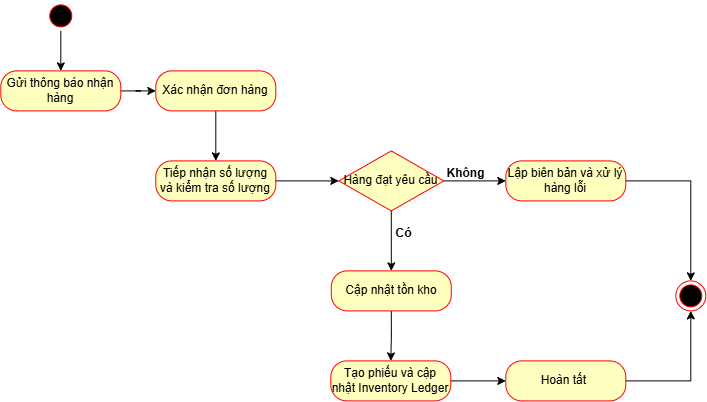
\includegraphics[
        width=0.92\textwidth,
        keepaspectratio
    ]{figures/Nhập hàng.png}
    \caption{Quy trình nhập hàng}
    \label{fig:workflow-purchase}
\end{figure}

\section{Quy trình bán hàng tại POS}

Quy trình bán hàng tại POS gồm tìm kiếm sản phẩm, kiểm tra tồn kho, giữ hàng,
xác nhận giao dịch và cập nhật tồn kho.

\begin{figure}[H]
    \centering
    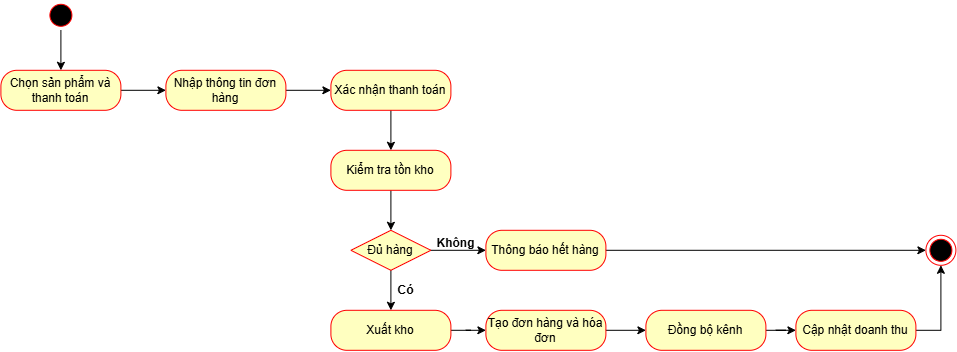
\includegraphics[
        width=0.92\textwidth,
        keepaspectratio
    ]{figures/bán POS.png}
    \caption{Quy trình bán hàng tại POS}
    \label{fig:workflow-pos}
\end{figure}

\section{Quy trình tiếp nhận đơn hàng đa kênh}

Đơn hàng từ các kênh bán hàng được tiếp nhận và đưa về mô hình đơn hàng thống nhất
trước khi xử lý.

\begin{figure}[H]
    \centering
    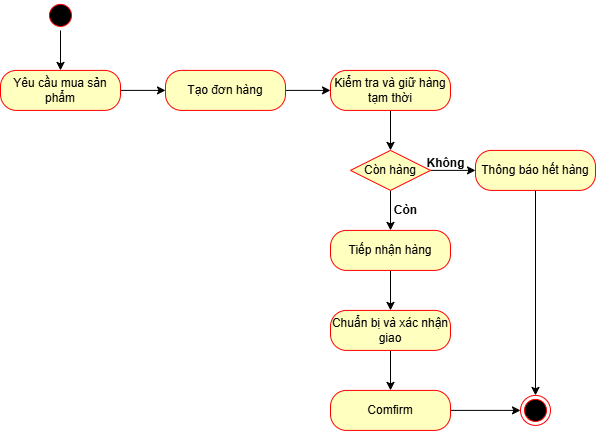
\includegraphics[
        width=0.92\textwidth,
        keepaspectratio
    ]{figures/nhận hàng.png}
    \caption{Quy trình tiếp nhận đơn hàng đa kênh}
    \label{fig:workflow-omnichannel}
\end{figure}

\section{Quy trình giữ hàng}

Hệ thống kiểm tra số lượng có thể bán trước khi giữ hàng cho đơn.
Nếu số lượng không đủ, yêu cầu giữ hàng bị từ chối.

\begin{figure}[H]
    \centering
    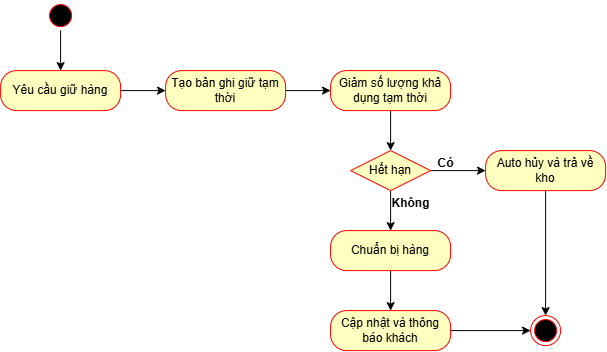
\includegraphics[
        width=0.92\textwidth,
        keepaspectratio
    ]{figures/giuhang.png}
    \caption{Quy trình giữ hàng}
    \label{fig:workflow-reservation}
\end{figure}

\section{Quy trình xuất kho và hoàn tất đơn hàng}

Sau khi đơn hàng được xác nhận, hàng hóa được xuất kho và đơn hàng chuyển sang trạng thái
hoàn tất theo quy trình nghiệp vụ.

\begin{figure}[H]
    \centering
    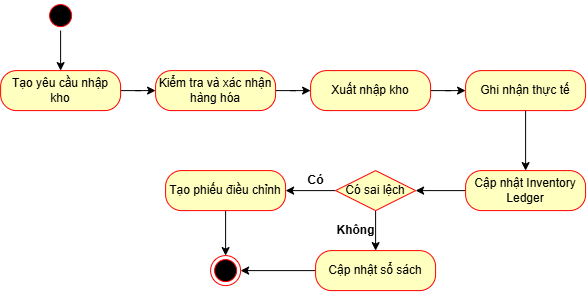
\includegraphics[
        width=0.92\textwidth,
        keepaspectratio
    ]{figures/nhapkho.png}
    \caption{Quy trình xuất kho và hoàn tất đơn hàng}
    \label{fig:workflow-deduct}
\end{figure}

\section{Quy trình hủy đơn}

Khi đơn hàng bị hủy, phần hàng đã giữ được giải phóng để có thể tiếp tục được bán
cho các đơn hàng khác.

\begin{figure}[H]
    \centering
    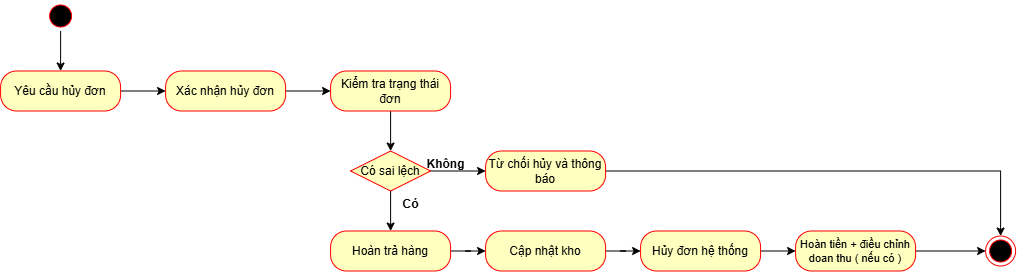
\includegraphics[
        width=0.92\textwidth,
        keepaspectratio
    ]{figures/huydon.png}
    \caption{Quy trình hủy đơn}
    \label{fig:workflow-cancel}
\end{figure}
